%%%%%%%%%%%%%%%%%%%%%%%%%%%%%%%%%%%%%%%%%
% Beamer Presentation
% LaTeX Template
% Version 1.0 (10/11/12)
%
% This template has been downloaded from:
% http://www.LaTeXTemplates.com
%
% License:
% CC BY-NC-SA 3.0 (http://creativecommons.org/licenses/by-nc-sa/3.0/)
%
%%%%%%%%%%%%%%%%%%%%%%%%%%%%%%%%%%%%%%%%%
% Content created by Shane Reynolds
% 16/08/2017
%%%%%%%%%%%%%%%%%%%%%%%%%%%%%%%%%%%%%%%%%

%----------------------------------------------------------------------------------------
%	PACKAGES AND THEMES
%----------------------------------------------------------------------------------------

\documentclass{beamer}

\mode<presentation> {

% The Beamer class comes with a number of default slide themes
% which change the colors and layouts of slides. Below this is a list
% of all the themes, uncomment each in turn to see what they look like.

%\usetheme{default}
%\usetheme{AnnArbor}
%\usetheme{Antibes}
%\usetheme{Bergen}
%\usetheme{Berkeley}
%\usetheme{Berlin}
%\usetheme{Boadilla}
%\usetheme{CambridgeUS}
%\usetheme{Copenhagen}
%\usetheme{Darmstadt}
%\usetheme{Dresden}
%\usetheme{Frankfurt}
%\usetheme{Goettingen}
%\usetheme{Hannover}
%\usetheme{Ilmenau}
%\usetheme{JuanLesPins}
%\usetheme{Luebeck}
\usetheme{Madrid}
%\usetheme{Malmoe}
%\usetheme{Marburg}
%\usetheme{Montpellier}
%\usetheme{PaloAlto}
%\usetheme{Pittsburgh}
%\usetheme{Rochester}
%\usetheme{Singapore}
%\usetheme{Szeged}
%\usetheme{Warsaw}

% As well as themes, the Beamer class has a number of color themes
% for any slide theme. Uncomment each of these in turn to see how it
% changes the colors of your current slide theme.

%\usecolortheme{albatross}
\usecolortheme{beaver}
%\usecolortheme{beetle}
%\usecolortheme{crane}
%\usecolortheme{dolphin}
%\usecolortheme{dove}
%\usecolortheme{fly}
%\usecolortheme{lily}
%\usecolortheme{orchid}
%\usecolortheme{rose}
%\usecolortheme{seagull}
%\usecolortheme{seahorse}
%\usecolortheme{whale}
%\usecolortheme{wolverine}

%\setbeamertemplate{footline} % To remove the footer line in all slides uncomment this line
%\setbeamertemplate{footline}[page number] % To replace the footer line in all slides with a simple slide count uncomment this line

%\setbeamertemplate{navigation symbols}{} % To remove the navigation symbols from the bottom of all slides uncomment this line
}

\usepackage{graphicx} % Allows including images
\usepackage{booktabs} % Allows the use of \toprule, \midrule and \bottomrule in tables
\usepackage[absolute,overlay]{textpos}
\usepackage{xfrac}
\usepackage{tcolorbox}
\usepackage{siunitx}
\usepackage{tikz}
  \setlength{\TPHorizModule}{1mm}
  \setlength{\TPVertModule}{1mm}

% The graphics path is relative to the .tex file
\graphicspath{{./figs/}}

% Graphics library in use for tikz
\usetikzlibrary{arrows}

% Add the university logo to the presentation
\addtobeamertemplate{frametitle}{}{%
\begin{textblock*}{100mm}(.85\textwidth,-0.25cm)
\includegraphics[scale=0.25]{logo.png}
\end{textblock*}}
%------------------------------------------------
%	TITLE PAGE
%------------------------------------------------

\title[Basics of Data Analysis]{Basics of Data Analysis} % The short title appears at the bottom of every slide, the full title is only on the title page

\author{} % Your name
\institute[Charles Darwin University] % Your institution as it will appear on the bottom of every slide, may be shorthand to save space
{
School of Engineering \\ % Your institution for the title page
\medskip
\textit{} % Your email address
}
\date{\today} % Date, can be changed to a custom date

\begin{document}

\begin{frame}
\titlepage % Print the title page as the first slide
\begin{textblock}{20}(80,30)
      \includegraphics[scale=0.8]{logo_1.png}
\end{textblock}
\end{frame}


%------------------------------------------------
%	PRESENTATION SLIDES
%------------------------------------------------

\begin{frame}
\frametitle{Introduction}
\begin{itemize}
\item This is a 2 hour workshop which is intended to serve as an introduction to data analysis.
\vspace{0.3cm}
\item The workshop does not provide an exhaustive exploration of all facets of data analytics.\\
\vspace{0.3cm}
\item In the interests of brevity, the workshop will cover some key points on the following topics:\\
\vspace{0.2cm}
\begin{enumerate}
\item Collecting Data
\vspace{0.2cm}
\item Storing and Manipulating Data
\vspace{0.2cm}
\item Creating Effective Graphs
\vspace{0.2cm}
\item Inference and Statistical Testing
\vspace{0.2cm}
\item Elementary Ordinary Least Squares Regresssion (OLS)
\end{enumerate}
\end{itemize}
\end{frame}

%------------------------------------------------

\begin{frame}
\frametitle{Stucture of the Workshop}
\begin{table}
\begin{tabular}{l l}
\toprule
\textbf{Section} & \textbf{Time}\\
\midrule
Collecting Data & 5 min\\
Storing \& Manipulating Data & 5 min\\
Creating Effective Pictures & 5 min\\
Activity 1 & 15 min\\
Statistical Analysis & 15 min\\
Activity 2 & 10 min\\
Ordinary Least Squares Regression & 15 min\\
Activity 3 & 10 min\\
\bottomrule
\end{tabular}
\end{table}
\end{frame}

%------------------------------------------------

\begin{frame}
\frametitle{Software for Examples}
There are a number of different analysis software packages that you can use. A few of the more popular packages are: 
\begin{columns}[b]
\column{0.65\textwidth}
\begin{figure}
\includegraphics[height=2cm]{R}
\end{figure}
\column{0.5\textwidth}
\includegraphics[height=2cm]{python}
\end{columns}
\vspace{0.5cm}
We will be using:
\begin{figure}
\includegraphics[height=3cm]{MATLAB-Logo}
\end{figure}
\end{frame}

%------------------------------------------------

\begin{frame}
\frametitle{Collection of Data}
\textbf{Measurement: Precision and Accuracy}\\
\vspace{0.5cm}
When collecting data in a scientific context we take measurements. There are 2 important aspects when looking at measurements: \textbf{precision} and \textbf{accuracy}
\vspace{0.5cm}
\begin{block}{Definition: \textbf{Accuracy}}
\textbf{Accuracy} refers to the closeness of a measured value to a standard or known value.
\end{block}
\begin{example}
In lab you obtain a weight measurement of 3.2 kg for a given substance, but the actual or known weight is 10 kg, then your measurement is not accurate. In this case, your measurement is not close to the known value.
\end{example}
\end{frame}

%------------------------------------------------

\begin{frame}
\frametitle{Collection of Data}
\textbf{Measurement: Precision and Accuracy}\\
\vspace{0.5cm}
\begin{block}{Definition: \textbf{Precision}}
\textbf{Precision} refers to the closeness of two or more measurements to each other.
\end{block}
\vspace{0.5cm}
\begin{example}
If in a lab you weigh a given substance five times, and get 3.2 kg each time, then your measurement is very precise.
\end{example}
\vspace{0.5cm}
Precision is independent of accuracy. You can be very precise but inaccurate, as described above. You can also be accurate but imprecise.
\end{frame}

%------------------------------------------------

\begin{frame}
\frametitle{Collection of Data}
\textbf{Measurement: Precision and Accuracy}\\
\vspace{0.5cm}
\begin{figure}
\includegraphics[scale=0.5]{accuracy_and_precision}
\caption{Accuracy is how far away from the true value a measurement is, and precision is the degree to which repeated measurements under unchanged conditions show the same results}
\end{figure}
\end{frame}

%------------------------------------------------

\begin{frame}
\frametitle{Collection of Data}
\textbf{Measurement: Precision and Accuracy}\\
\vspace{0.5cm}
\begin{figure}
\includegraphics[scale=0.5]{precision_accuracy}
\end{figure}
\end{frame}

%------------------------------------------------

\begin{frame}[fragile]
\frametitle{Collection of Data}
\textbf{Measurement: Precision and Accuracy}\\
\vspace{0.1cm}
\begin{itemize}
\item Accuracy and precision are dependent on the instrument used to take measurements
\vspace{0.1cm}
\item Good science will report the \textbf{accuracy} and the \textbf{precision} of the instruments used to take measurements.
\vspace{0.1cm}
\end{itemize}
\begin{tcolorbox}
\textbf{Finding the Absolute Accuracy of an Instrument}
\begin{enumerate}
\item Find a known value of the phenomena you are measuring, $V_A$
\item Take a measurement of the phenomena using the instrument, $V_O$
\item Use the following formula to determine the percentage error:
\begin{align*}
\epsilon = \frac{V_O - V_A}{V_A} \times 100\%
\end{align*}
\end{enumerate}
\end{tcolorbox}
\end{frame}

%------------------------------------------------

\begin{frame}[fragile]
\frametitle{Collection of Data}
\textbf{Measurement: Precision and Accuracy}\\
\vspace{0.1cm}
\begin{tcolorbox}
\textbf{Estimating the Precision of an Instrument}
\begin{enumerate}
\item  
\item 
\item 
\end{enumerate}
\end{tcolorbox}
\vspace{0.5cm}
It is important to note that the \textbf{precision} and \textbf{accuracy} are normally given in the data sheet that accompanies your instrument.\\
\vspace{0.5cm}
Some examples of sentence starters for reporting your precision and accuracy are:
\begin{itemize}
\item
\item
\end{itemize}

\end{frame}

%------------------------------------------------

\begin{frame}
\frametitle{Collection of Data}
\textbf{The Importance of Collecting Data on an Experimental Control}\\
\vspace{0.5cm}
A controlled experiment often compares the results obtained from experimental samples against \textbf{control samples}.\\
\vspace{0.5cm}
\textbf{Control Samples} are practically identical to the experimental sample except for the one aspect whose effect is being tested (the independent variable).
\end{frame}

%------------------------------------------------

\begin{frame}
\frametitle{Collection of Data}
\textbf{Understanding the Domain of your Dependant Variables}\\
\vspace{0.2cm}
\begin{itemize}
\item Try to have some understanding of the domain you want to investigate for your dependent variables.
\vspace{0.1cm}
\item Perhaps even collect data for some margin beyond the edges of these domains.
\vspace{0.1cm}
\item This foresight will help you to avoid extrapolation in your analysis - extrapolation is bad science.
\end{itemize}
\begin{figure}
\includegraphics[scale=0.35]{extrap}
\end{figure}
\end{frame}

%------------------------------------------------

\begin{frame}
\frametitle{Storing and Manipulating Data}
\textbf{Keep Data Storage and Data Analysis Separate}\\
\vspace{0.2cm}
\begin{block}{Definition: \textbf{Data Storage}}
\textbf{Data storage} simply means recording each observation made.
\end{block}
\begin{block}{Definition: \textbf{Data Analysis}}
\textbf{Data analysis} means creating graphics, tables or using statistics to uncover patterns or relationships in the data.
\end{block}  
\begin{figure}
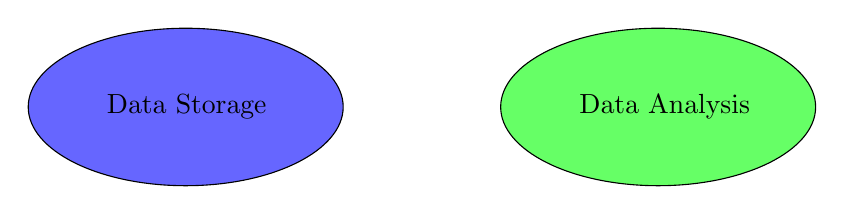
\begin{tikzpicture}
\draw [fill=blue!60] (-3,0) ellipse (2cm and 1cm);
\draw [fill=green!60] (3,0) ellipse (2cm and 1cm);
\node[text width=3cm] at (-2.5,0) {Data Storage};
\node[text width=3cm] at (3.5,0) {Data Analysis};
\end{tikzpicture}
\caption{Think of these two tasks as separate non-overlapping domains - combining the two can make your analysis inflexible, or end up creating extra work for yourself.}
\end{figure}
\end{frame}

%------------------------------------------------

\begin{frame}
\frametitle{Storing and Manipulating Data}
\textbf{Keep Data Storage and Data Analysis Separate}
\vspace{0.5cm}
\begin{figure}
\includegraphics[scale=0.33]{bad_structure}
\caption{An example of mixing these two domains}
\end{figure}
\end{frame}

%------------------------------------------------

\begin{frame}
\frametitle{Storing and Manipulating Data}
\textbf{How Should I Structure My Data?}
\vspace{0.5cm}
\begin{block}{Definition: \textbf{Observation}}
\textbf{Observation} refers to any data collected during the scientific activity.
\end{block}
\vspace{0.5cm}
\begin{block}{Definition: \textbf{Variable}}
A \textbf{variable} is any factor, trait, or condition that can exist in differing amounts or types.
\end{block}
\vspace{0.5cm}
When collecting your data, one good practice is to record your data in a matrix array with each \textbf{row} representing an observation, and each \textbf{column} representing a variable.
\end{frame}

%------------------------------------------------

\begin{frame}
\frametitle{Storing and Manipulating Data}
\textbf{How Should I Structure My Data?}
\vspace{0.5cm}
\begin{figure}
\begin{tikzpicture}
\node[anchor=south west,inner sep=0] at (0,0) {\frame{\includegraphics[scale=0.22]{titanic}}};
\draw[->,thick,blue] (-0.5,4.3) -- (-0.5,0) node [pos=0.5,above,font=\footnotesize,rotate=90] {observations};
\draw[->,thick,red] (0,4.8) -- (10,4.8) node [pos=0.5,above,font=\footnotesize] {variables};
\end{tikzpicture}
\caption{In this matrix array, each \textbf{\textcolor{blue}{observation}} is recorded in a \textbf{\textcolor{blue}{row}}, and each \textbf{\textcolor{red}{variable}} is listed over a \textbf{\textcolor{red}{column}}.}
\end{figure}
\end{frame}

%------------------------------------------------

\begin{frame}
\frametitle{Storing and Manipulating Data}
\textbf{How Should I Structure My Data?}\\
\vspace{0.5cm}
\begin{figure}
\includegraphics[scale=0.33]{bad_structure}
\caption{This is a bad way to structure your data set}
\end{figure}
\end{frame}

%------------------------------------------------

\begin{frame}
\frametitle{Storing and Manipulating Data}
\textbf{How Should I Structure My Data?}\\
\vspace{0.5cm}
\begin{figure}
\includegraphics[scale=0.33]{good_structure}
\caption{This is the data set on the previous slide reformatted to make it more readily usable for exploration and analysis}
\end{figure}
\end{frame}

%------------------------------------------------

\begin{frame}
\frametitle{Storing and Manipulating Data}
\textbf{Manipulating Data: Large Datasets}\\
\vspace{0.5cm}
\begin{itemize}
\item Large datasets will need to be manipulated in a software package like MATLAB
\vspace{0.5cm}
\item Large datasets typically arise from scientific instruments that sample at high frequencies
\vspace{0.5cm}
\item Do not try to manage large datasets in a spreadsheet application - this will be unwieldy, and provide little insight
\vspace{0.5cm}
\item Take some time to understand how to work with your dataset in your chosen software package - each package will have its own quirks
\end{itemize}
\end{frame}

%------------------------------------------------

\begin{frame}
\frametitle{Storing and Manipulating Data}
\textbf{Manipulating Data: Medium Datasets}\\
\vspace{0.5cm}
\begin{itemize}
\item You can manipulate a medium size data set directly in a software package like MATLAB, however, this is often clunky and can make basic visualisation of your data a pain.
\vspace{0.2cm}
\item An easier way to manipulate data is with a spreadsheet software package, like Excel or Google Sheets.
\vspace{0.2cm}
\item The main advantage of using a spreadsheet software is that it will make visualising your data set easier, and it is very simple to save as a \textbf{.csv} file which you can then import to an analysis software package.
\vspace{0.2cm}
\item \textbf{NOTE: this slide is not suggesting that you should undertake exploration or analysis of your dataset in a spreadsheet. Often these applications are ill-equipped to perform the exploration or analysis that you require}
\end{itemize}
\end{frame}

%------------------------------------------------

%\begin{frame}
%\frametitle{Storing and Manipulating Data}
%\textbf{What Format Should I Use To Save My Data?}\\
%\vspace{0.2cm}
%There are many formats in which you can save data, but %\textbf{.csv}\\ (comma separated values) is one of the %easiest to work with and is widely supported by many %software packages.
%\begin{figure}
%\includegraphics[scale=0.33]{csv}
%\caption{A .csv file separates values by commas and is %ubiquitously supported by analysis software packages}
%\end{figure}
%\end{frame}

%------------------------------------------------

\begin{frame}[fragile]
\frametitle{Storing and Manipulating Data}
\textbf{Tips for Storing Data: Large Datasets}\\
\vspace{0.5cm}
\begin{itemize}
\item Combining large datasets from two or more different experiments will most likely not be helpful
\vspace{0.5cm}
\item When you save your data sets make sure you use an appropriate naming convention, for example:
\begin{center}
\verb|experiment_<number of experiment>_<yyyymmdd>|
\end{center}
\vspace{0.5cm}
\item Using a naming convention like the one above will automatically keep you files in order
\end{itemize}
\end{frame}
%------------------------------------------------

\begin{frame}[fragile]
\frametitle{Storing and Manipulating Data}
\textbf{Tips for Storing Data: Medium Datasets}\\
\vspace{0.5cm}
\begin{itemize}
\item Don't be afraid to add redundant information to your master file - it may help with your analysis later.
\vspace{0.5cm}
\item Try to have only one data file called your \textbf{master}, this may mean adding extra variables like \textit{date}. \textbf{Note: never delete any of your data files - even after combining them into a single data file}
\vspace{0.5cm}
\item When you update your master file, you should not overwrite the old one - this will help to provide some version control. A good naming convention would be:
\begin{center}
\verb|master_<yyyymmdd>|
\end{center}
\end{itemize}
\end{frame}

%------------------------------------------------

\begin{frame}
\frametitle{Creating Effective Pictures}
\textbf{Why Use Graphs?}
\vspace{0.5cm}
\begin{itemize}
\item Data analysis is a process, which can be split up into three main operations:
\begin{enumerate}
\item \textbf{Collection:} collecting data, obviously
\item \textbf{Exploration:} uncovering patterns, trends, and gathering corroborative evidence to support arguments
\item \textbf{Analysis:} using statistics to make inferential claims
\end{enumerate}
\vspace{0.5cm}
\item One of the key tools to help explore the data is to use graphs
\vspace{0.5cm}
\item Graphs can help you find corroborative evidence for your hypotheses, and can be used to help strengthen arguments
\vspace{0.5cm}
\item Graphs can also be used to help you uncover patterns or relationships which may not be initially evident
\end{itemize}
\end{frame}

%------------------------------------------------

\begin{frame}
\frametitle{Creating Effective Pictures}
\textbf{To Plot or Not to Plot?}\\
\vspace{0.2cm}
\begin{itemize}
\item The purpose of plotting scientific data is to visualise variation or show relationships between variables
\vspace{0.5cm}
\item Not all data sets require a plot
\vspace{0.5cm}
\item If there are only one or two points, it is easy to examine the numbers directly - little or nothing is gained by putting them on a graph
\vspace{0.5cm}
\item Similarly, if there is no variation in the data, it is easy enough to see or state the fact without using a graph of any sort.
\end{itemize}
\end{frame}

%------------------------------------------------

\begin{frame}
\frametitle{Creating Effective Pictures}
\textbf{Graphing: The Fundamentals}\\
\vspace{0.1cm}
\begin{itemize}
\item Ensure that you are \textbf{labelling your axes} and including the \textbf{units of measurement} on these axes - many thesis submissions neglect this aspect
\item Every figure has a caption placed beneath it that describes the content in a few lines
\item The caption usually starts with a sequential figure number that is used for reference elsewhere in the paper. 
\end{itemize}
\vspace{-0.2cm}
\begin{figure}
\includegraphics[scale=0.3]{graph_example}
\vspace{-0.2cm}
\caption{A caption will help to explain what the figure is about}
\end{figure}
\end{frame}

%------------------------------------------------

\begin{frame}
\frametitle{Creating Effective Pictures}
\textbf{Graphing: The Fundamentals}\\
\vspace{0.5cm}
\begin{itemize}
\item A legend in the form of a text box in the plot area is sometimes used to identify the symbols associated with each data set.
\vspace{0.5cm}
\item If present, the legend must be placed in the plot area so that it does not detract from the display of data.
\vspace{0.5cm}
\item In formal technical publications legend information is often placed in the caption, but a legend may be useful for other presentations such as posters or talks.
\end{itemize}
\end{frame}

%------------------------------------------------

\begin{frame}
\frametitle{Creating Effective Pictures}
\textbf{Graphing: The Fundamentals}\\
\vspace{0.2cm}
When a graph is appropriate, it must be of an appropriate type to avoid misleading the reader.
\begin{figure}
\includegraphics[scale=0.45]{bad_graph}
\end{figure}
\vspace{-0.5cm}
\begin{itemize}
\item Both plots above show US research expenditures by discipline in 2000.
\item The scatter plot on the left is incorrect - it suggests a relationship between the variables on the two axes implied by the connecting lines.
\item The horizontal axis is just a list of disciplines with no inherent ordering, no relationship can exist.
\end{itemize}
\end{frame}
%------------------------------------------------

\begin{frame}
\frametitle{Creating Effective Pictures}
\textbf{Choosing the Right Graph (Small Dataset)}\\
\vspace{0.2cm}
\begin{itemize}
\item There is a limited amount of choice when it comes to plotting small data sets
\vspace{0.2cm}
\item In fact, some plots of small data sets can be misleading and promote erroneous conclusions
\end{itemize}
\vspace{-0.2cm}
\begin{figure}
\includegraphics[scale=0.08]{small_data}
\vspace{-0.2cm}
\caption{A plot which can work for small data sets is plotting the mean, maximum, and minimum value, however, be wary of drawing any strong conclusions from these graphs}
\end{figure}
\end{frame}
%------------------------------------------------

\begin{frame}
\frametitle{Creating Effective Pictures}
\textbf{Choosing the Right Graph (Med. \& Large Dataset): Distributions}\\
\vspace{0.2cm}
A picture can significantly aid the process of describing the distribution of your data for a variable.
\begin{figure}
\begin{tabular}{l p{6cm}}
\toprule
\textbf{Type of Graph} & \textbf{Appropriate Use}\\
\midrule
Histogram & Used with continuous and some discrete variables\\
 & \\
Box Plot & Used with continuous and discrete variables\\
 & \\
Ordered Bar Charts & Used when an ordinal metric can be placed on a categorical variable\\
\bottomrule
\end{tabular}
\end{figure}
\end{frame}

%------------------------------------------------

\begin{frame}
\frametitle{Creating Effective Pictures}
\textbf{Choosing the Right Graph (Med. \& Large Dataset): Distributions}\\
\vspace{0.2cm}
\begin{itemize}
\item A histogram works well for a continuous variable
\vspace{0.1cm}
\item A histogram can also work for some discrete variables
\vspace{0.1cm}
\item Histograms should be avoided for categorical variables
\vspace{0.1cm}
\item Be judicious when choosing your bin size - the wrong choice can reduce the effectiveness of your histogram
\end{itemize}
\vspace{-0.1cm}
\begin{figure}
\includegraphics[scale=0.25]{histogram}
\vspace{-0.4cm}
\caption{An example of a histogram}
\end{figure}
\end{frame}

%----------------------------------------------------

\begin{frame}
\frametitle{Creating Effective Pictures}
\textbf{Choosing the Right Graph (Med. \& Large Dataset): Distributions}\\
\begin{itemize}
\item If your bin size is too big you risk all of your data falling into only one or two categories
\vspace{0.2cm}
\item If you bin size is too small, you risk only one observation falling into each bin
\vspace{0.2cm}
\item Both of these situations will yield bad histograms 
\end{itemize}
\vspace{-0.2cm}
\begin{figure}
\includegraphics[scale=0.27]{histogram_bin}
\vspace{-0.3cm}
\caption{Most software packages will choose an optimal bin size for you}
\end{figure}
\end{frame}

%----------------------------------------------------

\begin{frame}
\frametitle{Creating Effective Pictures}
\textbf{Choosing the Right Graph (Med. \& Large Dataset): Distributions}\\
\vspace{0.2cm}
\begin{itemize}
\item A \textbf{box plot} is a concise way to show the distribution of data
\vspace{0.1cm}
\item These plots are generally very effective when comparing the distributions of two or more data sets for a variable
\vspace{0.1cm}
\item \textbf{Box plots} are very useful for showing how a distribution changes over time
\end{itemize}
\vspace{-0.1cm}
\begin{figure}
\frame{\includegraphics[scale=0.3]{box_plot}}
\caption{The key features of a \textbf{box plot}}
\end{figure}
\end{frame}

%----------------------------------------------------

\begin{frame}
\frametitle{Creating Effective Pictures}
\textbf{Choosing the Right Graph (Med. \& Large Dataset): Distributions}\\
\vspace{0.2cm}
\begin{columns}[b]
\column{0.45\textwidth}
\begin{figure}
\includegraphics[scale=0.5]{boxplot_ex}
\caption{Mapping the \textbf{box plot} to a distribution}
\end{figure}
\column{0.5\textwidth}
\begin{figure}
\includegraphics[scale=0.35]{Box_scatter}
\caption{How a \textbf{box plot} maps to a skewed distribution}
\end{figure}
\end{columns}
\end{frame}

%----------------------------------------------------

\begin{frame}
\frametitle{Creating Effective Pictures}
\textbf{Choosing the Right Graph (Med. \& Large Dataset): Distributions}\\
\begin{figure}
\includegraphics[scale=0.6]{box_time}
\caption{An example showing how \textbf{box plots} can be used to explain a changing distribution over time}
\end{figure}
\end{frame}

%----------------------------------------------------

\begin{frame}
\frametitle{Creating Effective Pictures}
\textbf{Choosing the Right Graph (Med. \& Large Dataset): Distributions}\\
\vspace{0.3cm}
If your variable is categorical, but has an ordinal metric which can be applied to it, then a \textbf{bar chart} will effectively describe the distribution
\begin{figure}
\includegraphics[scale=0.4]{grade_dist_3}
\vspace{-0.3cm}
\caption{Grade data is categorical, but has an underlying order to it. The side by side graphs show a shift in the grade distribution}
\end{figure}
\end{frame}

%----------------------------------------------------
\begin{frame}
\frametitle{Creating Effective Pictures}
\textbf{Choosing the Right Graph (Med. \& Large Dataset): Scatter Plots}\\
\vspace{0.2cm}
\begin{itemize}
\item Scatter plots can give you an idea of the relationship between two variables - a great precursor to a regression analysis
\vspace{0.2cm}
\item Scatter plots work really well for continuous variables
\vspace{0.2cm}
\item One variable is on the $x$-axis, another variable is on the $y$-axis, and each point in the Cartesian plane is an observation
\end{itemize}
\begin{figure}
\includegraphics[scale=0.3]{scatter}
\vspace{-0.5cm}
\caption{A scatter plot of two continuous variables}
\end{figure}
\end{frame}

%----------------------------------------------------
\begin{frame}
\frametitle{Creating Effective Pictures}
\textbf{Choosing the Right Graph (Med. \& Large Dataset): Scatter Plots}\\
\vspace{0.5cm}
Using scatter plots for \textbf{discrete data} can still be effective, but can be a bit tricky to get an effective picture because observations can overlap each other
\vspace{-1cm}
\begin{columns}[t]
\column{0.45\textwidth}
\begin{figure}
\includegraphics[scale=0.3]{scatter_1}
\caption{A scatter plot of discrete data}
\end{figure}
\column{0.45\textwidth}
\begin{figure}
\includegraphics[scale=0.3]{scatter_2}
\caption{A better scatter plot of discrete data - each observation carries a 0.1 visual weight, helping readers to better understand where observation locations}
\end{figure}
\end{columns}
\end{frame}

%----------------------------------------------------

\begin{frame}
\frametitle{Creating Effective Pictures}
\textbf{Choosing the Right Graph (Med. \& Large Dataset):\\ Two Datasets on One Graph?}\\
\vspace{0.2cm}
\begin{itemize}
\item There are very few situations where it is appropriate to use two different scales on the same plot
\vspace{0.2cm}
\item It is very easy to mislead the viewer of the graphic - this is bad science
\end{itemize}
\vspace{-0.4cm}
\begin{columns}
\column{0.45\textwidth}
\begin{figure}
\includegraphics[scale=0.2]{2plot_1}
\vspace{-0.3cm}
\caption{The intersecting plots seem to imply something}
\end{figure}
\column{0.5\textwidth}
\begin{figure}
\includegraphics[scale=0.2]{2plot_2}
\vspace{-0.3cm}
\caption{A simple change of scale reveals the original plot is misleading}
\end{figure}
\end{columns}
\end{frame}

%----------------------------------------------------

\begin{frame}
\frametitle{Creating Effective Pictures}
\begin{figure}
\large\textbf{It's now time to attempt activity 1}
\end{figure}
\end{frame}

%----------------------------------------------------
\begin{frame}
\frametitle{Statistical Analysis}
\textbf{What is this section about?}\\
\vspace{0.5cm}
This section of the workshop is really only about three things:
\vspace{0.4cm}
\begin{itemize}
\item Understanding \textbf{population parameters}, \textbf{sample statistics}, and the \textbf{sampling distribution of means};
\vspace{0.4cm}
\item How you can \textbf{estimate population parameters} using \textbf{confidence intervals}
\vspace{0.4cm}
\item Understanding how to correctly set up a \textbf{hypothesis test}, why you might like to do this, and when this statistical analysis is appropriate;
\end{itemize}
\end{frame}

%----------------------------------------------------
\begin{frame}
\frametitle{Statistical Analysis}
\textbf{Populations and Samples}
\vspace{0.2cm}
\begin{figure}
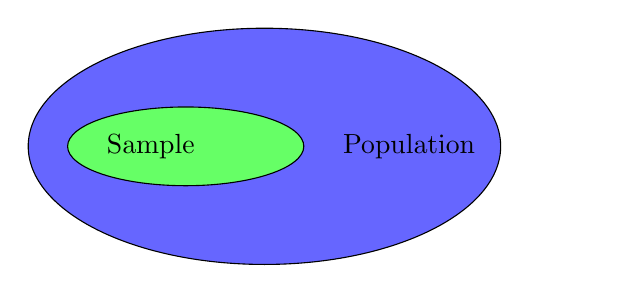
\begin{tikzpicture}
\draw [fill=blue!60] (0,0) ellipse (3cm and 1.5cm);
\draw [fill=green!60] (-1,0) ellipse (1.5cm and 0.5cm);
\node[text width=3cm] at (-0.5,0) {Sample};
\node[text width=3cm] at (2.5,0) {Population};
\end{tikzpicture}
\caption{A sample is a small set of a population}
\end{figure}
\vspace{-1cm}
\begin{columns}[t]
\column{0.45\textwidth}
\begin{block}{Definition: \textbf{Population}}
A \textbf{population} is a set of similar items or event which is of some interest for some question or experiment
\end{block}
\column{0.5\textwidth}
\begin{block}{Definition: \textbf{Sample}}
A \textbf{sample} is a set of data collected from a statistical population
\end{block}
\end{columns}
\end{frame}

%----------------------------------------------------
\begin{frame}
\frametitle{Statistical Analysis}
\textbf{Parameters and Statistics}
\begin{columns}[t]
\column{0.45\textwidth}
\begin{block}{Definition: \textbf{Parameter}}
A \textbf{parameter} is any summary number, like an average or percentage, that describes the entire \textbf{population}.
\end{block}
\column{0.5\textwidth}
\begin{block}{Definition: \textbf{Statistic}}
A \textbf{statistic} is any summary number, like an average or percentage, that describes a \textbf{sample}.
\end{block}
\end{columns}
\begin{table}
\caption{Shows the correct notation used to represent parameters and statistics}
\begin{tabular}{l c c }
\toprule
 & Population & Sample\\
 & Parameter & Statistic\\
 \midrule
 Mean & $\mu$ & $\bar{x}$\\
 Standard Deviation & $\sigma$ & $s$\\
 \bottomrule
\end{tabular}
\end{table}
\end{frame}

%----------------------------------------------------
\begin{frame}
\frametitle{Statistical Analysis}
\textbf{The Sampling Distribution of Means}
\vspace{0.2cm}
\begin{block}{Definition: \textbf{Continuous Random Variable}}
A \textbf{continuous random variable}, usually denoted as $X$, is a variable whose value is assigned from a set of possible outcomes according to some probability distribution.
\end{block}
\vspace{0.4cm}
\begin{itemize}
\item Suppose we start taking samples from some population defined by a random variable $X$
\vspace{0.4cm}
\item For each of these samples we calculate the mean, $\bar{x}$
\vspace{0.4cm}
\item Each $\bar{x}$ will be different due to sampling variability
\end{itemize}
\end{frame}

%----------------------------------------------------
\begin{frame}
\frametitle{Statistical Analysis}
\textbf{The Sampling Distribution of Means}
\begin{figure}
\scalebox{0.6}{
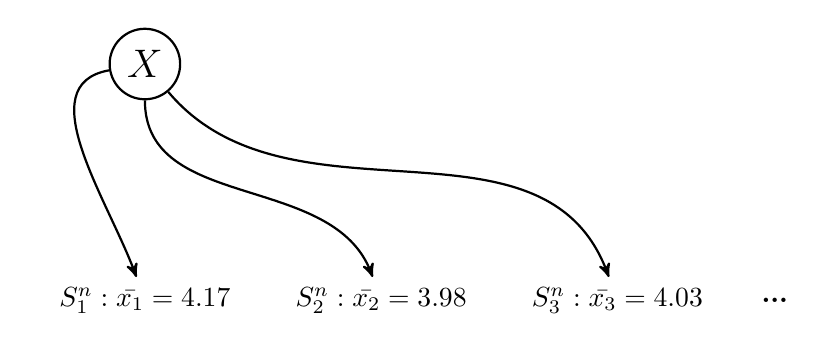
\begin{tikzpicture}
  [
    ->,
    >=stealth',
    auto,node distance=3cm,
    thick,
    main node/.style={circle, draw, font=\sffamily\Large\bfseries}
    ]

  \node (1) {$S_1^n: \bar{x_1}=4.17$};
  \node (2) [right of=1] {$S_2^n: \bar{x_2}=3.98$};
  \node (3) [right of=2] {$S_3^n: \bar{x_3}=4.03$};
  \node (4) [right of=3, node distance=2cm] {\textbf{...}};
  \node [main node] (5) [above of=1] {$X$};

  \draw (5) [out=190, in=110] to  (1);
  \draw (5) [out=270, in=110] to  (2);
  \draw (5) [out=310, in=110] to  (3);
\end{tikzpicture}
}
\vspace{-0.3cm}
\caption{Samples of size $n$, denoted by $S_i^n$, are taken from the population represented by random variable $X$. The distribution of $X$ is unknown, but it has some true mean $\mu$, and some true standard deviation $\sigma$. For each sample the mean, $\bar{x_i}$, is calculated.}
\end{figure}
\vspace{-0.3cm}
\begin{itemize}
\item The sample means form a distribution of their own, $\overline{X}$
\vspace{0.1cm}
\item According to the central limit theorem, the sample means are normally distributed, that is $\overline{X} \sim N(\mu_{\bar{x}},\sigma_{\bar{x}})$
\vspace{0.1cm}
\end{itemize}
\end{frame}

%----------------------------------------------------
\begin{frame}
\frametitle{Statistical Analysis}
\textbf{The Sampling Distribution of Means}\\
\vspace{0.5cm}
\begin{tcolorbox}
If the sample size, $n$, is big enough then,
\begin{align*}
	\overline{X} \sim N(\mu_{\bar{x}},\sigma_{\bar{x}})
\end{align*}
This is true \textbf{irrespective} of whether or not $X$ is normally distributed.
\end{tcolorbox}
\begin{itemize}
\item The mean of the sample means is the true population mean, that is:
\begin{align*}
\mu_{\bar{x}} = \mu
\end{align*}
\item The standard deviation of the sample means, also called the \textit{standard error}, is given by:
\begin{align*}
 \sigma_{\bar{x}} = \frac{\sigma}{\sqrt{n}}
\end{align*}
\end{itemize}
\end{frame}

%----------------------------------------------------
\begin{frame}
\frametitle{Statistical Analysis}
\textbf{The t-distribution}\\
\vspace{0.5cm}
\begin{itemize}
\item Statistical test should be done using $z$-scores if the population parameter, $\sigma$ , is known
\vspace{0.5cm}
\item The problem with this is that we often don't know the true population parameter $\sigma$
\vspace{0.5cm}
\item Additionally if our underlying distribution is not normal and our sample is too small, then we can get erronous results from inference
\vspace{0.5cm}
\item What do we do instead?
\vspace{0.5cm}
\item \textbf{Use the $t$-distribution}
\end{itemize}
\end{frame}

%----------------------------------------------------
\begin{frame}
\frametitle{Statistical Analysis}
\textbf{The t-distribution}\\
\vspace{0.1cm}
If the population parameter, $\sigma$, is unknown, or the sample size is less than 30, then: 
\begin{itemize}
\item We use the sample statistic $s$ to approximate $\sigma$; and
\item The normal distribution is abandoned in favour of the student's $t$-distribution
\end{itemize}
\vspace{0.1cm}
\begin{tcolorbox}
The key conditions to check prior to using the $t$-distribution:\\
\vspace{-0.5cm}
\begin{itemize}
\item When \textbf{sample size is less than 15}, use t-distribution only when population is very close to normal
\vspace{0.1cm}
\item When \textbf{sample size is between 15 and 30}, the $t$-distribution can be used if the variable is not far from normal
\vspace{0.1cm}
\item When \textbf{sample size is large}, we can always use $t$-distribution provided there are no extreme outliers that cannot be removed
\end{itemize}
\end{tcolorbox}
\end{frame}

%----------------------------------------------------
\begin{frame}
\frametitle{Statistical Analysis}
\textbf{Inference}\\
\vspace{0.5cm}
Now that the justification for using the $t$-distribution has been covered, we turn our focus to inference which relies on $t$-scores.\\
\vspace{0.3cm}
\textbf{NOTE: these inference techniques also work for $z$-scores, if they are appropriate to use}
\vspace{0.5cm}
\begin{block}{Definition: \textbf{Inference}}
Statistical \textbf{inference} is the theory, methods, and practice of forming judgements about the parameters of a population.
\end{block}
\vspace{0.5cm}
We will look at two forms of inference:
\begin{itemize}
\item Estimating population means using confidence intervals
\item Hypothesis testing
\end{itemize}
\end{frame}
%----------------------------------------------------
\begin{frame}
\frametitle{Statistical Analysis}
\textbf{Estimating the Population Mean Using Confidence Intervals}\\
\vspace{0.2cm}
\begin{itemize}
\item Suppose we want to estimate an actual population mean $\mu$ - we may only be able to obtain $\bar{x}$, the mean of a sample randomly selected from the population of interest
\vspace{0.2cm}
\item We can use $\bar{x}$ to find a range of values:
\begin{align*}
\textrm{Lower value}<\mu<\textrm{Upper value}
\end{align*}
\item This range of values provides us with some confidence that it contains the population mean μ
\vspace{0.2cm}
\item The range of values is called a \textbf{confidence interval}
\end{itemize}
\begin{block}{Defintion: \textbf{Confidence Interval}}
A \textbf{confidence interval} is a range of values so defined that there is a specified probability that the value of a parameter lies within it.
\end{block}
\end{frame}

%----------------------------------------------------
\begin{frame}
\frametitle{Statistical Analysis}
\textbf{Estimating the Population Mean Using Confidence Intervals}\\
\vspace{0.2cm}
\begin{itemize}
\item We are interested in finding a (1-$\alpha$)100\% confidence interval for the population mean $\mu$, where $0< |\alpha| < 1$
\vspace{0.2cm}
\item The formula for the confidence interval in words is:
\vspace{-0.3cm}
\begin{align*}
\textrm{Sample mean} \pm (\textrm{t-multiplier} \times \textrm{standard error})
\end{align*}
\end{itemize}
\vspace{-0.3cm}
\begin{tcolorbox}
The formula for the \textbf{confidence interval} in notation is:
\begin{align*}
\bar{x} \pm t_{\alpha/2,n-1} \cdot \frac{s}{\sqrt{n}}
\end{align*}
\end{tcolorbox}
\vspace{0.1cm}
The \textit{$t$-multiplier}, which we denote as $t_{\alpha/2,n-1}$, depends on the sample size through $n-1$ (called the \textit{degrees of freedom}), and the confidence level $(1-\alpha) \times 100$ through $\alpha/2$.
\end{frame}

%----------------------------------------------------

\begin{frame}
\frametitle{Statistical Analysis}
\textbf{Estimating the Population Mean Using Confidence Intervals}\\
\vspace{0.2cm}
\begin{example}
Example of confidence interval calculation using t distribution
\end{example}
\end{frame}

%----------------------------------------------------

\begin{frame}
\frametitle{Statistical Analysis}
\textbf{Hypothesis Testing}\\
\vspace{0.5cm}
\begin{tcolorbox}
The general idea of \textbf{hypothesis testing} involves:
\vspace{0.2cm}
\begin{enumerate}
\item Making an initial assumption
\vspace{0.2cm}
\item Collecting evidence (data)
\vspace{0.2cm}
\item Based on the available evidence (data), deciding whether to reject or not reject the initial assumption
\end{enumerate}
\end{tcolorbox}
\vspace{0.2cm}
Every hypothesis test — regardless of the population parameter involved — requires the above three steps.
\end{frame}

%----------------------------------------------------

\begin{frame}
\frametitle{Statistical Analysis}
\textbf{Hypothesis Testing}\\
\begin{example}
\textbf{Is normal body temperature really 36.67$\si{\degreeCelsius}$?}\\
\vspace{0.1cm}
Consider the population of many adults. A researcher wants an answer to the question: "Is the average adult body temperature 36.67$\si{\degreeCelsius}$?" To answer his research question, the researcher starts by assuming that the average adult body temperature was 36.67$\si{\degreeCelsius}$.\\
\vspace{0.1cm}
Then, the researcher goes out and tries to find evidence that refutes his initial assumption. In doing so, he selects a random sample of 130 adults. The average body temperature of the 130 sampled adults is 37.81$\si{\degreeCelsius}$.\\
\vspace{0.1cm}
Then, the researcher uses the data he collected to make a decision about his initial assumption. It is either likely or unlikely that the researcher would collect the evidence he did given his initial assumption that the average adult body temperature is 36.67$\si{\degreeCelsius}$?
\end{example}
\end{frame}

%----------------------------------------------------

\begin{frame}
\frametitle{Statistical Analysis}
\textbf{Hypothesis Testing}\\
\begin{example}
\textbf{(Continued) Is normal body temperature really 36.67$\si{\degreeCelsius}$?}\\
\vspace{0.1cm}
If it is likely, then the researcher does not reject his initial assumption that the average adult body temperature is 36.67$\si{\degreeCelsius}$. There is not enough evidence to do otherwise.\\
\vspace{0.1cm}
If it is unlikely, then:
\begin{itemize}
\item either the researcher's initial assumption is correct and he experienced a very unusual event;
\item or the researcher's initial assumption is incorrect.
\end{itemize}
\vspace{0.1cm}
In the practice of statistics, if the evidence (data) we collected is unlikely in light of the initial assumption, then we reject our initial assumption.
\end{example}
\end{frame}

%----------------------------------------------------

\begin{frame}
\frametitle{Statistical Analysis}
\textbf{Hypothesis Testing}\\
\vspace{0.5cm}
\begin{itemize}
\item In statistics, we always assume the null hypothesis is true. That is, the null hypothesis is always our initial assumption.
\vspace{0.5cm}
\item In statistics, the data are the evidence.
\vspace{0.5cm}
\item In statistics, we always make one of two decisions:
\vspace{0.2cm} 
\begin{itemize}
\item We either \textbf{reject the null hypothesis}; or
\vspace{0.2cm}
\item We \textbf{fail to reject the null hypothesis}
\end{itemize}
\end{itemize}
\end{frame}

%----------------------------------------------------

\begin{frame}
\frametitle{Statistical Analysis}
\textbf{Steps for Hypothesis Testing}\\
\vspace{0.5cm}
\textbf{STEP 1 - Setting up two competing hypotheses}
\vspace{0.2cm}
\begin{itemize}
\item Each hypothesis test includes two hypothesis about the population
\vspace{0.2cm}
\item One is the null hypothesis, notated as $H_0$, which is a statement of a particular parameter value
\vspace{0.2cm}
\item This hypothesis is assumed to be true until there is evidence to suggest otherwise
\vspace{0.2cm}
\item The second hypothesis is called the alternative, or research, hypothesis, written as $H_a$
\vspace{0.2cm}
\item The alternative hypothesis is a statement of a range of alternative values in which the parameter may fall
\end{itemize}
\end{frame}

%----------------------------------------------------

\begin{frame}
\frametitle{Statistical Analysis}
\textbf{Steps for Hypothesis Testing}\\
\vspace{0.5cm}
\textbf{STEP 2 - Set some level of significance called alpha}
\vspace{0.2cm}
\begin{itemize}
\item This value is used as a probability cutoff for making decisions about the null hypothesis
\vspace{0.2cm}
\item The most common alpha value is 0.05  or 5\%. Other popular choices are 0.01 (1\%)
\end{itemize}
\vspace{0.2cm}
\textbf{STEP 3 - Calculate a test statistic}
\vspace{0.2cm}
\begin{itemize}
\item Gather sample data and calculate a test statistic where the sample statistic is compared to the parameter value
\vspace{0.2cm}
\item The test statistic is calculated under the assumption the null hypothesis is true
\end{itemize}
\end{frame}

%----------------------------------------------------

\begin{frame}
\frametitle{Statistical Analysis}
\textbf{Steps for Hypothesis Testing}\\
\vspace{0.3cm}
\textbf{STEP 4 - Calculate probability value (p-value)}
\vspace{0.2cm}
\begin{itemize}
\item A p-value is found by using the test statistic to calculate the probability of the sample data producing such a test statistic or one more extreme
\vspace{0.2cm}
\item A small p-value means that we reject the null hypothesis
\vspace{0.2cm}
\item A \textit{small p-value} means that the \textit{probability of getting this sample is low, assuming the null hypothesis is true} 
\end{itemize}
\vspace{0.2cm}
\textbf{STEP 5 - Make a test decision about the null hypothesis}
\vspace{0.2cm}
\begin{itemize}
\item In this step we decide to either reject the null hypothesis or decide to fail to reject the null hypothesis
\vspace{0.2cm}
\item Notice we do not make a decision where we will accept the null hypothesis
\end{itemize}
\end{frame}

%----------------------------------------------------

\begin{frame}[fragile]
\frametitle{Statistical Analysis}
\textbf{Steps for Hypothesis Testing}\\
\vspace{0.3cm}
\textbf{STEP 6 - State an overall conclusion}
\vspace{0.2cm}
\begin{itemize}
\item Once we have found the p-value, and made a statistical decision about the null hypothesis, we want to summarise our results into an overall conclusion for our test
\vspace{0.2cm}
\item Include a sentence starter on what you can say for rejection of null \verb|text|
\vspace{0.2cm}
\item Include a sentence starter on what you can say for failure to reject null \verb|text|
\end{itemize}
\end{frame}

%----------------------------------------------------

\begin{frame}
\frametitle{Statistical Analysis}
\textbf{Type I and Type II Errors}\\
\vspace{0.3cm}
When doing hypothesis testing, two types of mistakes may be made and we call them Type I error and Type II error.
\begin{figure}
\includegraphics[scale=0.4]{t1t2_error}
\caption{Table shows the errors that can be made when performing hypothesis testing}
\end{figure}
\vspace{-1cm}
\begin{itemize}
\vspace{0.2cm}
\item If we reject $H_0$ when $H_0$ is true, we commit a \textbf{Type I} error. The probability of Type I error is denoted by: $\alpha$.
\vspace{0.2cm}
\item If we fail to reject $H_0$ when $H_0$ is false, we commit a \textbf{Type II} error. The probability of Type II error is denoted by: $\beta$.
\end{itemize}
\end{frame}

%----------------------------------------------------

\begin{frame}
\frametitle{Statistical Analysis}
\textbf{One Sample t testing of a mean}\\
\vspace{0.3cm}
\end{frame}

%----------------------------------------------------

\begin{frame}
\frametitle{Statistical Analysis}
\textbf{Two Sample t testing of a mean}\\
\vspace{0.3cm}
\end{frame}

%----------------------------------------------------

\begin{frame}
\frametitle{Statistical Analysis}
\begin{figure}
\large\textbf{It's now time to attempt activity 2}
\end{figure}
\end{frame}

%----------------------------------------------------

\begin{frame}
\frametitle{Ordinary Least Squares (OLS) Regression}
\textbf{What is Ordinary Least Squares Regression}\\
\vspace{0.3cm}
\begin{itemize}
\item Ordinary least squares (OLS) is a method for estimating the unknown parameters in a linear regression model
\vspace{0.3cm}
\item It is one of the methods which we can assign a \textit{line of best fit} to a data set
\end{itemize}
\begin{columns}
\column{0.45\textwidth}
The linear regression model that would be fit to the data shown on the left, would be:
\begin{align*}
GDP(\% \Delta) = \beta_0 + \beta_1 \cdot UE(\% \Delta)
\end{align*}
OLS would determine the $\beta_0$, and $\beta_1$ coefficients.
\column{0.5\textwidth}
\begin{figure}
\includegraphics[scale=0.4]{regression}
\caption{A scatter plot showing unemployment vs. GDP}
\end{figure}
\end{columns}
\end{frame}

%----------------------------------------------------

\begin{frame}
\frametitle{Ordinary Least Squares (OLS) Regression}
\textbf{What is Ordinary Least Squares Regression}\\
\vspace{0.5cm}
\begin{itemize}
\item OLS is more than simply fitting a line to the data - it tests whether that relationship is statistically significant
\vspace{0.2cm}
\item Consider the model $y \sim \beta_0 + \beta_1 \cdot x$
\vspace{0.2cm}
\item When an OLS is run, it also performs the following statistical tests:
\begin{align*}
H_0: \beta_0 = 0 \quad\quad H_0: \beta_1 = 0\\
H_a: \beta_0 \neq 0 \quad\quad H_a: \beta_1 \neq 0
\end{align*}
\item p-values are reported for each of these tests
\end{itemize}
\end{frame}

%----------------------------------------------------

\begin{frame}
\frametitle{Ordinary Least Squares (OLS) Regression}
\textbf{What is Ordinary Least Squares Regression}\\
\vspace{1cm}
\begin{tcolorbox}
\begin{itemize}
\item \textbf{If the p-value is low} - it means the $x$ variable is statistically significant in explaining the $y$ variable
\vspace{0.5cm}
\item \textbf{If the p-value is high} - it means that the $x$ variable is not statistically significant in explaining the $y$ variable
\end{itemize}
\end{tcolorbox}
\end{frame}

%----------------------------------------------------

\begin{frame}
\frametitle{Ordinary Least Squares (OLS) Regression}
\textbf{Important Assumptions of OLS Regression}\\
\vspace{0.3cm}
\begin{itemize}
\item Many are familiar with using OLS to fit straight lines (or non-linear transformations) to data sets in their high school, undergraduate, or postgraduate careers
\vspace{0.3cm}
\item There are, however, some important assumptions that need to be satisfied if you want to use OLS to show the statistical significance of a relationship in your data
\vspace{0.3cm}
\item This workshop will consider the two most important assumptions:
\vspace{0.1cm}
\begin{itemize}
\item \textbf{Homoskedasticity assumption}
\vspace{0.1cm}
\item \textbf{No autocorrelation assumption}
\end{itemize}
\end{itemize}
\end{frame}

%----------------------------------------------------

\begin{frame}
\frametitle{Ordinary Least Squares (OLS) Regression}
\textbf{Important Assumptions: Homoskedasticity}\\
\vspace{0.3cm}
\begin{itemize}
\item The homoskedasticity assumption of the fitted model is that the standard deviations of the error terms are constant
\vspace{0.2cm}
\item If this assumption is \textbf{violated} it is \textbf{not appropriate to use OLS} to provide statistical evidence of a relationship
\vspace{0.2cm}
\item To test for homoskedasticity we look at the residual plot - we expect to see \textbf{no pattern in the residual plot}\vspace{0.2cm}
\item If there is no pattern in the residual plot, then we can assume that the homoskedasticity assumption has not been violated
\end{itemize}
\end{frame}

%----------------------------------------------------

\begin{frame}
\frametitle{Ordinary Least Squares (OLS) Regression}
\textbf{Important Assumptions: Homoskedasticity}\\
\vspace{0.3cm}
\begin{figure}
\includegraphics[scale=0.3]{homosked}
\caption{The residual plot on the right looks like a random scatter of the residuals - there is no apparent pattern in the residuals}
\end{figure}
\end{frame}
%----------------------------------------------------

\begin{frame}
\frametitle{Ordinary Least Squares (OLS) Regression}
\textbf{Important Assumptions: Autocorrelation}\\
\vspace{0.3cm}
\begin{block}{Definition: \textbf{Autocorrelation}}
\textbf{Autocorrelation}, also known as serial correlation, is the correlation of a signal with a delayed copy of itself.
\end{block}
\begin{itemize}
\item In OLS there is an assumption that there will be \textbf{no autocorrelation present in the residuals}
\vspace{0.2cm}
\item We can test for autocorrelation in the residuals once the model has been run
\vspace{0.2cm}
\item One type of data where autocorrelation is almost ALWAYS present is time series data
\vspace{0.2cm}
\item As a general rule, it is \textbf{not appropriate to use OLS regression with time series data}
\end{itemize}
\end{frame}

%----------------------------------------------------

\begin{frame}
\frametitle{Ordinary Least Squares (OLS) Regression}
\textbf{How to perform OLS Regression Using MATLAB}\\
\vspace{0.3cm}
\begin{tcolorbox}
\begin{enumerate}
\item Determine your model prior to fitting it to the data - it is bad science to look at the data first and then fit the model
\vspace{0.1cm}
\item Load your data into MATLAB
\vspace{0.1cm}
\item Fit your model using OLS
\vspace{0.1cm}
\item Check the residual plot to ensure that the homoskedasticty assumption is not violated
\vspace{0.1cm}
\item Perform a statistical test to ensure that there is no autocorrelation in the residuals
\vspace{0.1cm}
\item Read the summary report to determine if the $\beta$ coefficients are statistically significant to your model
\end{enumerate}
\end{tcolorbox}
\end{frame}

%----------------------------------------------------

\begin{frame}
\frametitle{Ordinary Least Squares (OLS) Regression}
\begin{figure}
\large\textbf{It's now time to attempt activity 3}
\end{figure}
\end{frame}

%----------------------------------------------------

\end{document} 